%!TEX program = xelatex
%!TEX TS-program = xelatex
%!TEX encoding = UTF-8 Unicode

\documentclass[a4paper]{article}
\usepackage[UTF8, heading = false, scheme = plain]{ctex}
\usepackage{graphicx}
\usepackage{cite}
\usepackage{geometry}
\geometry{left=2.0cm, right=2.0cm, top=2.5cm, bottom=2.5cm}
\usepackage[colorlinks,linkcolor=red,anchorcolor=blue,citecolor=green]{hyperref}
\usepackage{subfig}
\usepackage{caption}
\captionsetup{font={scriptsize}}

\renewcommand\figurename{图}

\makeatletter
\let\@afterindentfalse\@afterindenttrue
\@afterindenttrue
\makeatother
\setlength{\parindent}{2em}  

\linespread{1.4}
\setlength{\parskip}{0.5\baselineskip}

\title{学习汇报\\第十四周}
\author{熊凯亚}
\date{\today}

\begin{document}
\maketitle
本周主要看了Shokri发表在SP'17上的一篇文章:针对机器学习模型的会员推理攻击\cite{shokri2017membership}。这篇文章主要讲了如何通过会员推理攻击(membership inference attack)。会员推理攻击为:对模型进行黑盒访问,对于给定的数据记录,可以确定这个数据记录是否存在于模型的原始训练数据集种。Shokri等人利用机器学习的对抗性训练自己的推理模型,来识别目标模型对其所训练的输入与未训练的输入的预测之间的差异。本文使用Google Prediction API和 Amazon ML等Machine Learning as a Service的服务进行实验。

\section{引言}
本文训练了一个attack model,这个模型的目的就是去分辨对于训练中产生的输入和没有产生的输入目标模型的不同行为,也就是说本文将一个会员推理问题转变成了分类问题。

为了训练这个attack model,本文提出了一种影子训练技术shadow training technique。首先创建多个影子模型来模仿目标模型的行为,虽然我们对于目标模型的内部结构并不清楚,但是我们对于自己创建的影子模型的内部结构是非常清晰的。然后我们在影子模型的输出和标记的输入数据上继续训练attack model。

训练数据方面:对于影子模型的训练,由于接触不到原始的训练数据,我们需要为影子模型生成训练数据。本文讲了三种生成训练数据的方法:1. 使用黑盒访问目标模型来合成数据;2. 使用关于目标的训练数据集的统计数据。 3. 假定攻击者可以访问目标模型的训练数据集的潜在的有噪声的版本。总的来说,方法一并不假设关于目标模型训练数据的任何先验知识,方法二和方法三在推断之前仅允许攻击者对目标模型进行一次记录查询。

本文提出的攻击模型非常通用,它并不依赖于任何特定的数据集或者模型结构或训练算法。本文的实验部分采用Google和Amazon的机器学习模型训练服务,即使Google和Amazon没有对我们(客户)透露模型的学习算法和结果模型的结构,本文提出的会员推理攻击依然可以对给定的数据记录判断其是否属于目标模型的训练数据。


\section{问题陈述}

\begin{figure*}[!ht]
\begin{tabular}{cc}
\subfloat[攻击模型]{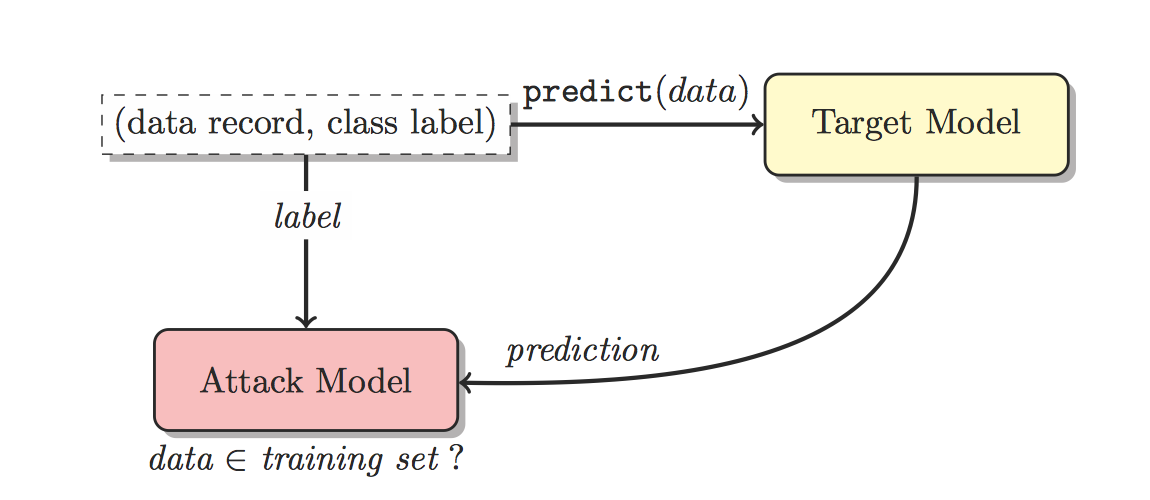
\includegraphics[width = 3.5in]{fig/blackbox.png}} &
\subfloat[训练模型]{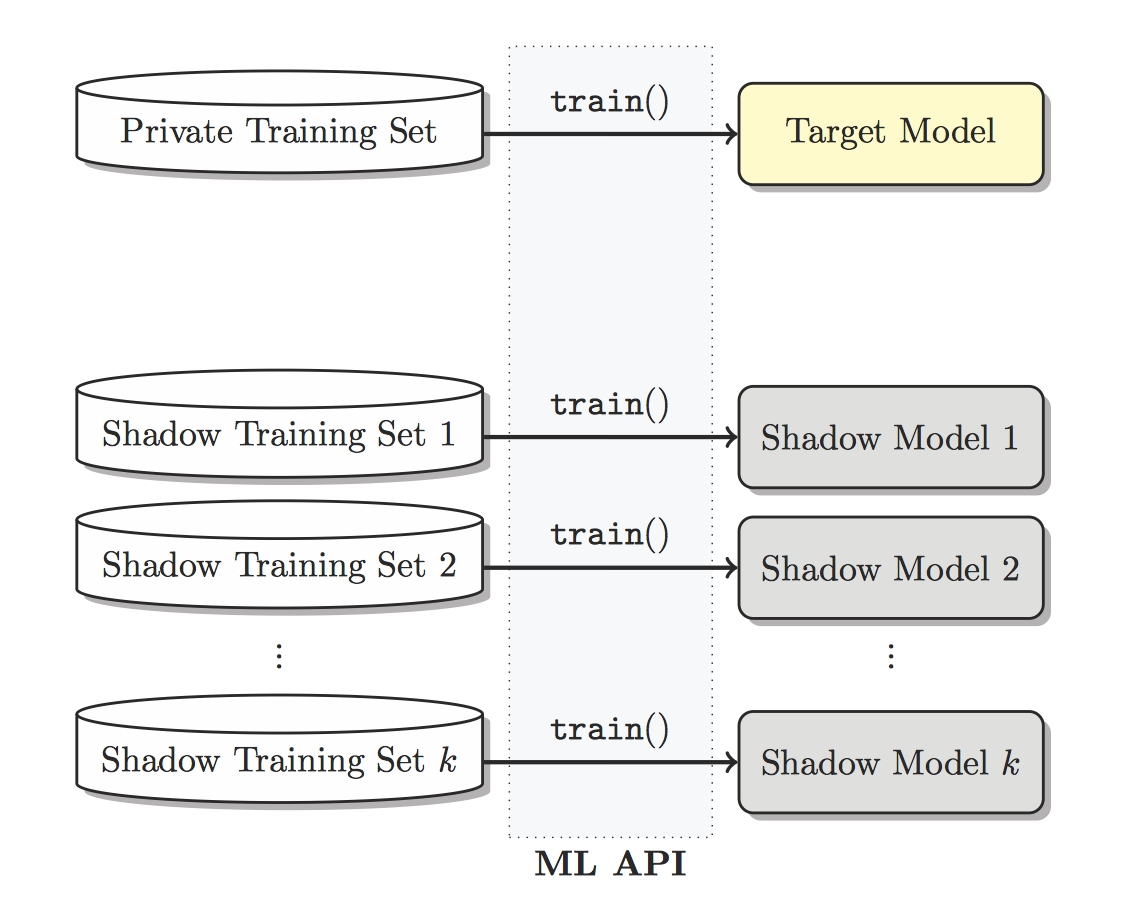
\includegraphics[width = 3.5in]{fig/mlapi.png}}
\end{tabular}
\caption{1. 攻击者使用数据记录查询目标模型获得模型在此记录的预测结果。2. ML API:使用于目标模型相同的训练服务(google or amazon)来训练影子模型。目标模型和影子模型的训练数据集的格式相同但是互不相交。影子模型之间的训练数据集可能会有重叠。所有模型的内部参数都独立训练。}
\end{figure*}

对于任何输入数据记录,该模型输出概率的预测向量,每个类输出一个表示这个记录属于某个特定类的预测向量概率。这个概率也被称为置信度。选择具有最高置信度值的类作为数据记录的预测标签。模型的准确性通过测量它如何在其训练集之外进行推广并预测来自同一群体的其他数据记录的标签来评估。

假设攻击者拥有对模型的查询访问权限,并可以在任何数据记录上获取模型的预测向量。攻击者知道模型的输入和输出的格式,包括它们的数量和值的范围。我们还假设攻击者:1.知道机器学习模型的类型和结构以及训练算法,或2.具有对机器学习的黑箱访问权限用于训练模型。在后一种情况下,攻击者不会事先知道模型的结构或元参数。


推理攻击的设置如下:攻击者用于目标模型的数据记录和黑盒查询访问权限。如果攻击者能够正确确定该数据记录是否是模型训练数据集的一部分,则攻击成功。攻击准确性的标准度量标准记为推理会员的记录中的一小部分真的是属于训练数据集。

\section{会员推理}

\subsection{总览}
机器学习模型对自己训练的数据和第一次见到的数据的行为不一样,其中过拟合是这种不一致的主要原因。而攻击者的目标就是构建一个可以识别在目标模型的行为中识别出这种不同的攻击模型,并利用它们仅依靠目标模型的输出从目标模型的训练集中识别出成员与非成员。

为了训练我们的攻击模型,我们构建了多个与目标模型行为类似的影子模型。与目标模型相反,我们知道每个影子模型的内部细节,即给定的记录是否在其训练数据集中。因此,我们可以对影子模型的输入和相应输出(每个标记为“in”或“out”)使用有监督的训练来训练攻击模型区分训练数据集成员的影子模型输出和它们的非成员输出。

\subsection{影子模型}
攻击者创建$k$个影子模型$f_{shadow}^i()$,每个模型的训练数据$D_{shadow}^{train}$的格式和分布都与目标模型的训练数据类似。我们假设用于训练影子模型的数据集和目标模型的训练数据集不相交,对于攻击者来说这是一种最坏的情况,如果两个数据集的数据有重叠的话,攻击的效果会更好。

影子模型必须以与目标模型相似的方式来训练,如果训练算法是一直的话这也很简单。但是Google Prediction API和Amazon ML等并不会告诉我们它们所使用的模型结构。但是我们可以通过与目标模型使用同一种“机器学习即服务”的服务来训练影子模型,以达到训练方式类似的效果。

\subsection{生成训练数据}
为了训练影子模型,我们需要与目标模型的训练数据分布类似的数据。

\paragraph{基于模型合成数据}
如果攻击者没有真实的训练数据或任何有关其分布的统计数据,他可以使用目标模型本身为影子模型生成合成训练数据。被高度置信度的目标模型分类的记录应该在统计上与目标的训练数据集相似,从而可以生成影子模型需要的训练数据。

综合过程分两个阶段进行:1. 搜索:使用hill-climbing算法搜索可能的数据范围,寻找目标模型高度置信分类的输入。2. 采样:从这些数据记录中抽取合成数据,重复这个过程直至训练数据集满。


这个过程只有在敌手能够有效地探索可能的输入空间并发现被高度置信的目标模型分类的输入时才起作用。例如,如果输入是高分辨率图像并且目标模型执行复杂的图像分类任务,则它可能不起作用。

\paragraph{基于统计合成数据}
攻击者可能拥有一些关于目标模型的训练数据所在的统计信息。例如,攻击者可能事先知道不同特征的边缘分布。在实验中,我们通过独立采样每个特征的边界分布值来生成影子模型的综合训练记录,实验表明,由此方式生成的数据攻击效果非常好。

\paragraph{噪音版的真实数据}
攻击者可以访问一些与目标模型的训练数据相似的数据,并且可以将其视为含有“噪音”的版本。在关于位置数据集的实验中,我们通过随机选择10%或20%的特征的(二值)来模拟,然后在产生的噪声数据集上训练影子模型。该场景模拟目标和影子模型的训练数据不是从完全相同的总体中采样,或者以非均匀方式采样的情况。

\subsection{训练攻击模型}

\begin{figure}
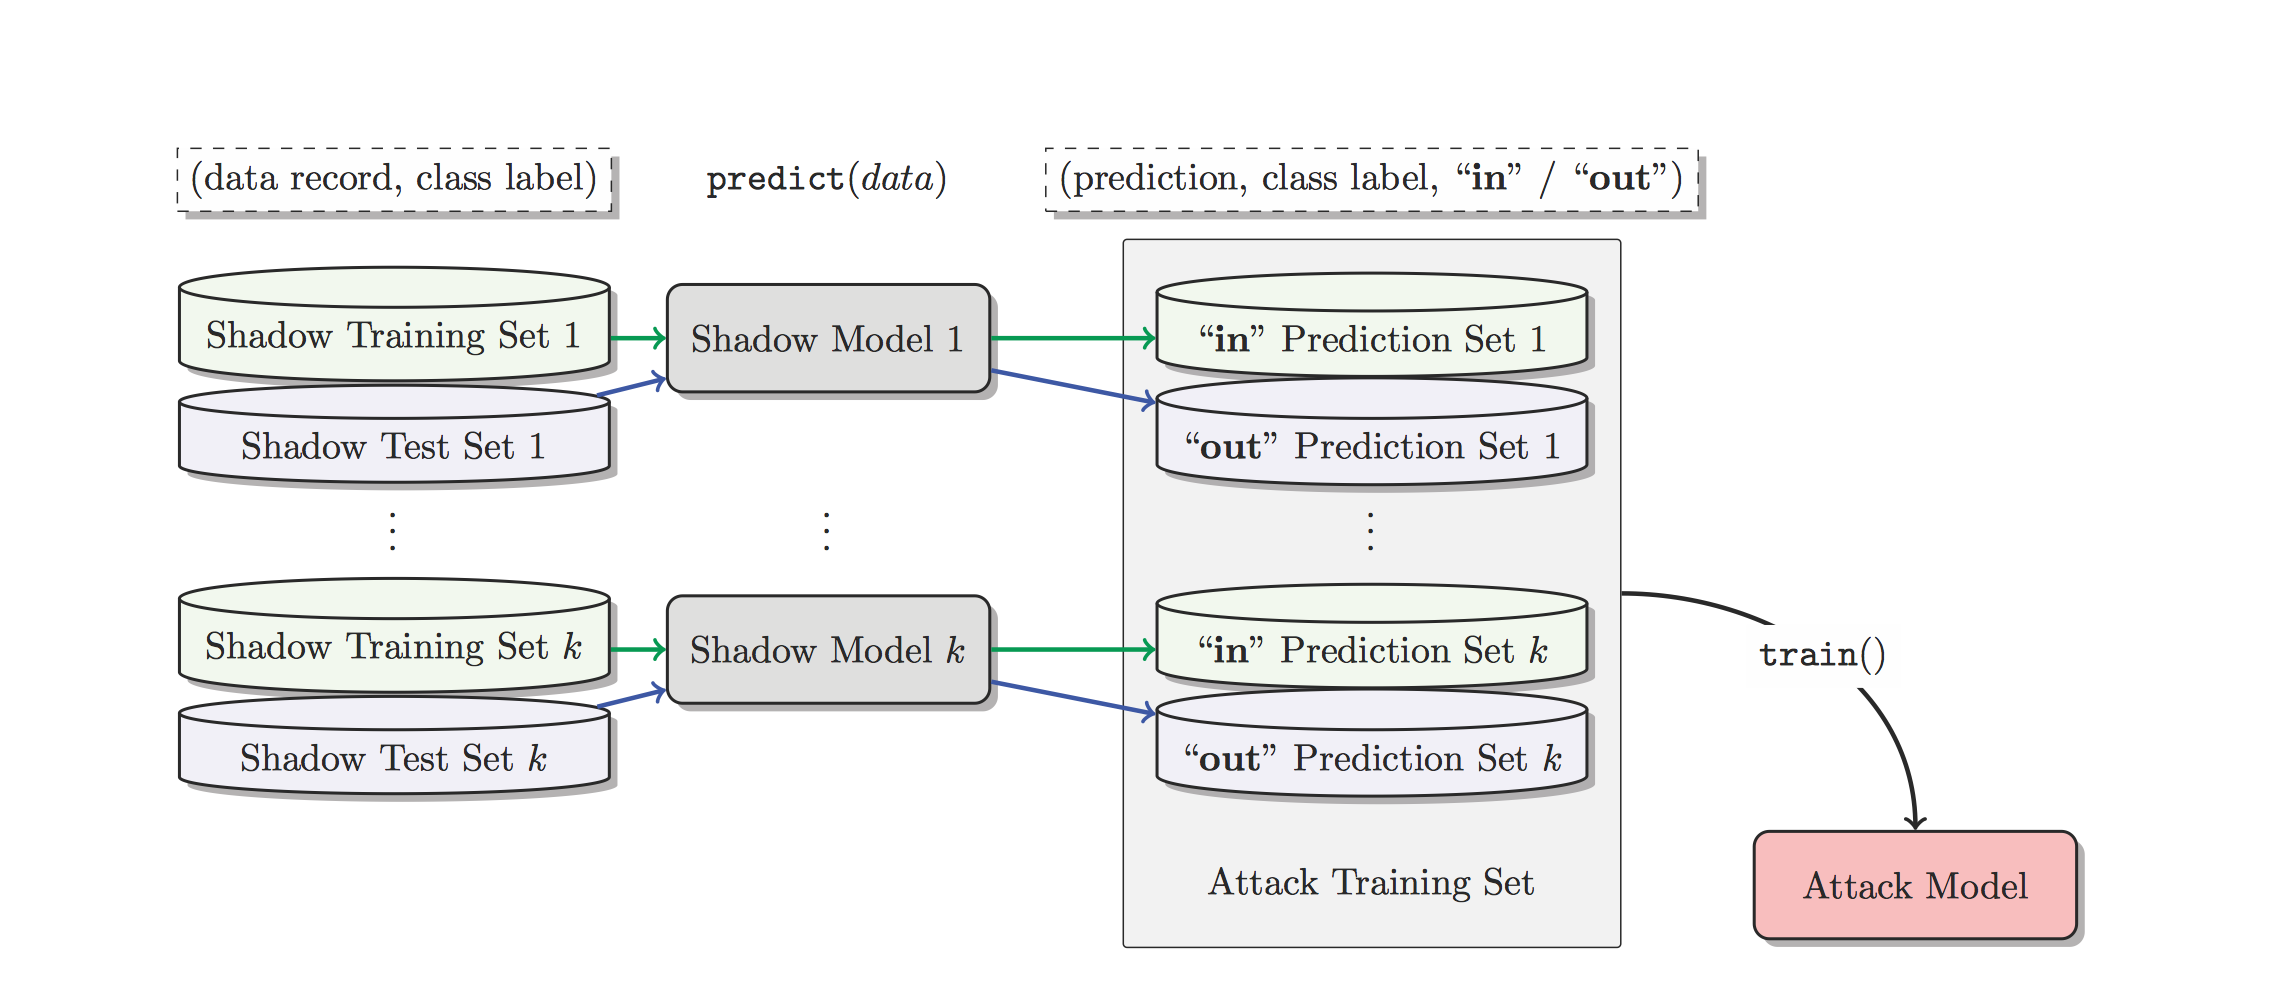
\includegraphics[width = \linewidth]{fig/training.png}
\caption{训练攻击模型对影子模型的输入和输出。对于影子模型训练数据集中的所有记录,查询模型并输出。这些输出向量被标记为$“in”$并添加到攻击模型的训练数据集。并且使用与训练数据集分离的测试数据集查询影子模型,该集合上的输出被标记为$“out”$,并添加到攻击模型的训练数据集。在构建一个数据集来反映影子模型在训练和测试数据集上的黑盒行为之后,训练了$c_{target}$个目标攻击模型的集合,每个目标模型的输出类都对应一个攻击模型。}
\end{figure}

影子训练技术背后的主要思想是,使用相同服务在类似数据记录上训练的类似模型的行为方式类似。这一观察结果在文章其余部分的实验中得到了验证。研究结果表明,学习如何推导影子模型训练数据集中的隶属度(我们知道一些关于影子模型的基本信息并可以在监督训练期间计算成本函数),从而产生一个成功推断目标模型训练数据集成员的攻击模型。

使用自己的训练数据集和相同大小的不相交测试集查询每个影子模型。训练数据集上的输出标记为$“in”$,其余标记为$“out”$。现在,攻击者拥有记录数据集,影子模型的相应输出以及输入/输出标签。攻击模型的目标是从记录和相应的输出中推断标签。

如果我们使用基于模型的训练数据合成方法,那么攻击模型的所有原始训练数据都是从目标模型中划分出来的,具有高置信度的记录。然而,这对于影子模型的训练数据集中使用的记录以及这些数据集中遗留的测试记录都是如此。因此,攻击模型并不是简单地学习识别被高度置信地分类的输入。相反,它学会执行一项更加微妙的任务:如何区分高置信度的训练输入和其他非高度置信的非训练输入。

本文将识别训练数据集成员与模型输出之间复杂关系的问题转化为二元分类问题。二分类是标准的机器学习任务,因此可以使用任何最先进的机器学习框架或服务来构建攻击模型。本文提出的方法独立于用于攻击模型训练的特定方法。例如,使用神经网络构建攻击模型,并使用本文正在攻击的黑盒Google Prediction API构建攻击模型,在这种情况下,我们无法控制模型结构,模型参数或训练元参数,但仍然可以获得有效的攻击模型。

\newpage
\bibliographystyle{IEEEtran}
\bibliography{references}
\end{document}
